\documentclass[12pt]{article}
\usepackage{verbatim}
\usepackage[dvips]{epsfig}
\usepackage{color}
\usepackage{url}
\usepackage[colorlinks=true]{hyperref}

\begin{document}

\section*{GENESIS: Documentation}

{\bf Related Documentation:}
% start: userdocs-tag-replace-items related-do-nothing
% end: userdocs-tag-replace-items related-do-nothing

\section*{Add a New Component to the {\it DeveloperPackage}}

GENESIS contains many software components. The source code of the most
important ones are publicly available from a central repository. (The
server {\tt repo-genesis3} is coded as the default server in
the \href{../developer-package/developer-package.tex}{\it DeveloperPackage}, 
a default that can be overwritten using command line
options.) Other software components can be made available from other
sources. The {\it DeveloperPackage}, when configured correctly,
automatically incorporates software components from geographically
distributed sources. The addition of a new software component to GENESIS is the equivalent to adding a new column to the associative array constructed by the {\it DeveloperPackage}. 

New software components can be added to the configuration of the {\it
  neurospaces\_build} script of the {\it DeveloperPackage}. All the other tools of the
{\it DeveloperPackage}, such as tools to compile and install, tools to synchronize
the source code with remote servers, and tools to generate and publish
documentation on a website will work with the new configuration.

For smooth integration with the GENESIS installer, it is a requirement that the top level source directory of the new component contains a {\it configure} script, and a {\it Makefile} with the targets {\it clean}, {\it check}, {\it dist}, {\it distcheck}, {\it install}, {\it uninstall}, {\it docs}, {\it html-upload-prepare}, {\it html-upload}, and {\it dist-keywords}.

\subsubsection*{Creating a new software component}

The following steps should be performed on your developer machine each time you wish to start development of a new software component.

Use the command line arguments ``{\tt --enable <your-software> --regex <your-software>}'' to limit the operations given below to only the software component named. Here, as an example, we use ``{\tt <your-software>}'' which should be replaced by the name of your software component. 

\begin{enumerate}
\item {\bf Add the new software component to the configuration of the {\it neurospaces\_build} script:} As an example, for the component named {\tt <your-software>}, you would add the following code block to the configuration file:
\begin{verbatim}
	'<your-software>' => {
	   './configure' => ['--with-delete-operation'],
	   directory => "$ENV{HOME}/neurospaces_project/<your-software>/source/snapshots/0",
	   disabled => 0,
	   order => 1,
	   target_name => '<your-software>',
	   version_control => {
	      port_number => 4693,
	      repository => "$ENV{HOME}/neurospaces_project/MTN/<your-software>.mtn",
	   },
},
\end{verbatim}
  This code block includes the directory name where sources are to be
  found, the build order, and version control information ({\bf Note:}
  the server port number cannot be changed at anytime). The {\tt \$} indicates a terminal prompt.

\item {\bf Create the correct directory layout:}
\begin{verbatim}
   $ neurospaces_create_directories
\end{verbatim}
  
\item {\bf Create the monotone repository:}
\begin{verbatim}
   $ neurospaces_init
\end{verbatim}

\item {\bf Populate the new project with files:} Use monotone to check in your modifications regularly (see \href{../version-control/version-control.tex}{\bf Version\,Control} for more details).

\end{enumerate}

\subsubsection*{Making a new software component available to others}

Serving the source code over the internet makes it available to
others.  It is best, although not required, to employ a dedicated user on
your machine to serve the source code.

\begin{itemize}
\item {\bf Configure your new monotone server:} The information in the
  configuration of the new software component is used by the {\it
    neurospaces\_serve} command to make the source code available over
  the internet.  If you are only serving your own software component,
  use the ``{\tt --enable <your-software> --regex <your-software>}''
  command line arguments.
  
\item {\bf Synchronize your private monotone repository:} After the
  server has been configured the developer package tools can be used to
  synchronize your private changes with the server, provided all tools
  have been configured with the updated configuration for
  {\tt <your-software>}.  For example, {\it neurospaces\_sync} can be used
  to synchronize your private repository with the server repository.
\end{itemize}
  
\subsubsection*{Pushing the new software component to other computers}

The following steps will enable others to access your new software.

\begin{itemize}

\item {\bf Get a version of the developer package that contains the
    configuration for the new software component.}
  
\item {\bf Create the correct directory layout:}
\begin{verbatim}
	neurospaces_create_directories
\end{verbatim}

\item {\bf Create the private monotone repository:} This step is
  optional because the pull operation in the next step will create a
  new repository for the new software component if required.
\begin{verbatim}
	neurospaces_init
\end{verbatim}

\item {\bf Pull the repository from the server:}
\begin{verbatim}
	neurospaces_pull --enable <your-software> \
	   --regex <your-software>
\end{verbatim}
  
\item {\bf Update local source code with the latest source in the
    local repository, keeping local changes if any:}
\begin{verbatim}
	neurospaces_update --enable <your-software> \
	   --regex <your-software>
\end{verbatim}
  
\item {\bf Recompile all software components, and link them against
    each other:}
\begin{verbatim}
	neurospaces_install --configure
\end{verbatim}
  The ``{\tt --configure}'' argument enables configuration, which is
  needed for a new software component.
\end{itemize}

To extend the functionality of a pre-existing GENESIS {\bf Component} see \href{../genesis-extend-model-container/genesis-extend-model-container.tex}{\bf Extending the Model\,Container}.

To extend the functionality of GENESIS by adding a new {\bf Component} see \href{../genesis-add-object-solver/genesis-add-object-solver.tex}{\bf Add Solver Object}.

\subsection*{Detailed Example}

As a modeling project grows, it may become necessary to create and maintain a new software component. We now show in detail how to add a new software component to the {\it DeveloperPackage} as well as how to create the corresponding monotone repository on a repository server. For this example, we will be adding a new package called the {\it exchange} package.

\subsubsection*{Adding a new component to the {\it DeveloperPackage}}

To add a new package to the system you must first make the script {\it neurospaces\_build} aware of your package. First locate the package matrix in {\it neurospaces\_build}:
\begin{verbatim}
   my $all_packages
\end{verbatim}
Next we must add an entry for our package, first we must designate a port number for performing {\it push}, {\it pull}s and {\it sync}s. The current port numbers in use range between 4692 ({\bf N S-SLI}) to 4700 ({\it userdocs}), so it is safe to designate port 4701 as the port for the {\it exchange} package.

{\bf WARNING:} Make absolutely certain that no two packages point to the same port number. Two packages attempting to {\it sync} to the same port number can result in a corruption of your repository.

Now we add our entry complete with port number:
\begin{verbatim}
   exchange => {
      dependencies => {
         'model-container' => 'for storing the model in computer memory',
      },
      directory => "$ENV{HOME}/neurospaces_project/exchange/source/snapshots/0",
      order => 1.5,
      version_control => {
         port_number => 4701,
         repository => "$ENV{HOME}/neurospaces_project/MTN/exchange.mtn",
      },
      version_script => 'neurospaces_exchange --version',
    },
\end{verbatim}
Here we add an entry to the package matrix (a Perl hash) with the following attributes.
\begin{itemize}
   \item {\bf dependencies:} List of package dependencies with a string message delimited by commas.
   \item {\bf directory:} The target directory for checking out source code.
   \item {\bf order:} A weight value which designates the order to perform pulls, pushes and syncs in
   \item {\bf version\_control:} Designates the port number and mtn file to use for version control
   \item {\bf version\_script:} Command to give the version number. 
\end{itemize}

\subsubsection*{Creating a new repository on the server}

For more context regarding the central server setup, see \href{../installation-debian-server/installation-debian-server.tex}{\bf Installation\,Debian\,Server}.

In this scenario a user has created the {\it exchange} package and wants to share the code by propagating it via the central repository. There are three machines:
\begin{itemize}
   \item {\bf User1:} Created the {\it exchange} package and has a monotone repository on their machine they'd like to share.
   \item {\bf User2:} Another user which would like to have access to the {\it exchange} package.
   \item {\bf repo:} A centralized server that serves the monotone repositories. 
\end{itemize}
First the the administrator of the repo initializes a new repository in the same location indicated in the directory hash from the values in the package matrix from {\it neurospaces\_build}. As the dedicated monotone user on the repo we execute this command to create a blank repository:
\begin{verbatim}
   mtn --db=~/neurospaces_project/MTN/exchange.mtn
\end{verbatim}
Next we need to add the public keys for {\tt User1} and {\tt User2} to the blank repository. To add their public keys you must first obtain them either via a secure transfer (encrypted email or {\it im}) or you can get it from a pre-existing repository via a command like this:
\begin{verbatim}
   mtn --db=~/neurospaces_project/MTN/heccer.mtn pubkey user1@email.com >~/user1.pubkey
\end{verbatim}
Once they're in files you can read them into the blank exchange repository:
\begin{verbatim}
   cat ~/user1.pubkey ~/user2.pubkey | mtn --db=~/neurospaces_project/MTN/exchange.mtn read
\end{verbatim}
Now with the blank repository in place with the users public keys, the {\it exchange} package can be served via {\it neurospaces\_serve} as well as {\it sync}ed and {\it pull}ed via {\it neurospaces\_sync} and {\it neurospaces\_pull} respectively. With the modified {\it neurospaces\_build} from the previous section installed on all of the users machines we can serve the repositories on the repo via:
\begin{verbatim}
   sudo -H -u monotone nohup neurospaces_serve &
\end{verbatim}
So the code sharing scenario can be illustrated like this:

\begin{figure}[h]
\centering
   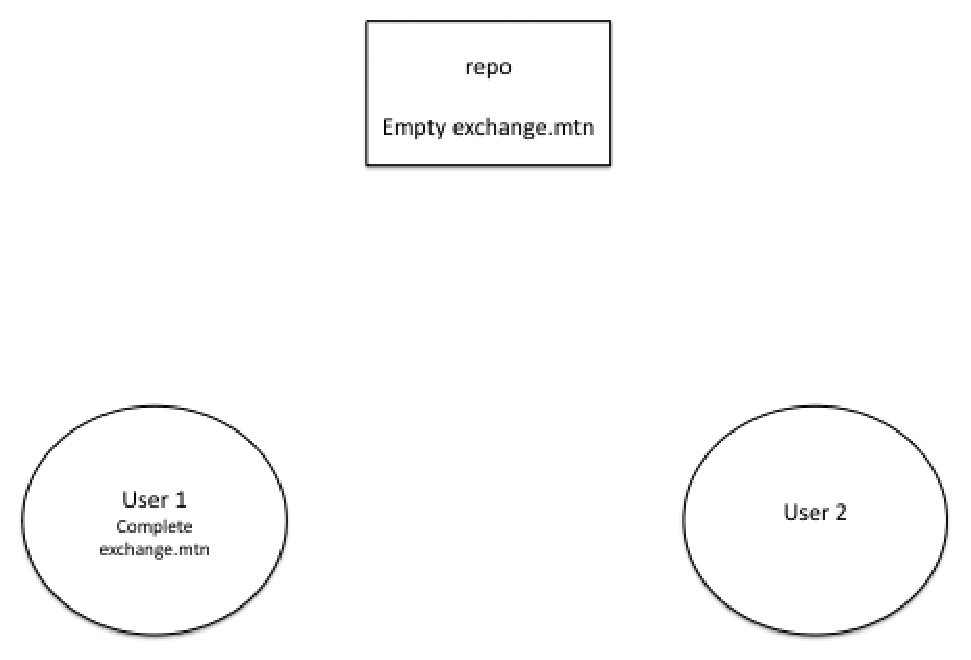
\includegraphics[scale=0.5]{figures/repo1.eps}
%   \caption{ }
   \label{fig:R1}
\end{figure}

{\tt User1} has the complete set of code in his repository for the exchange package. The repo serves an empty repository on a designated port for the exchange package. {\tt User 2} has no repository or code yet.

\begin{figure}[h]
\centering
   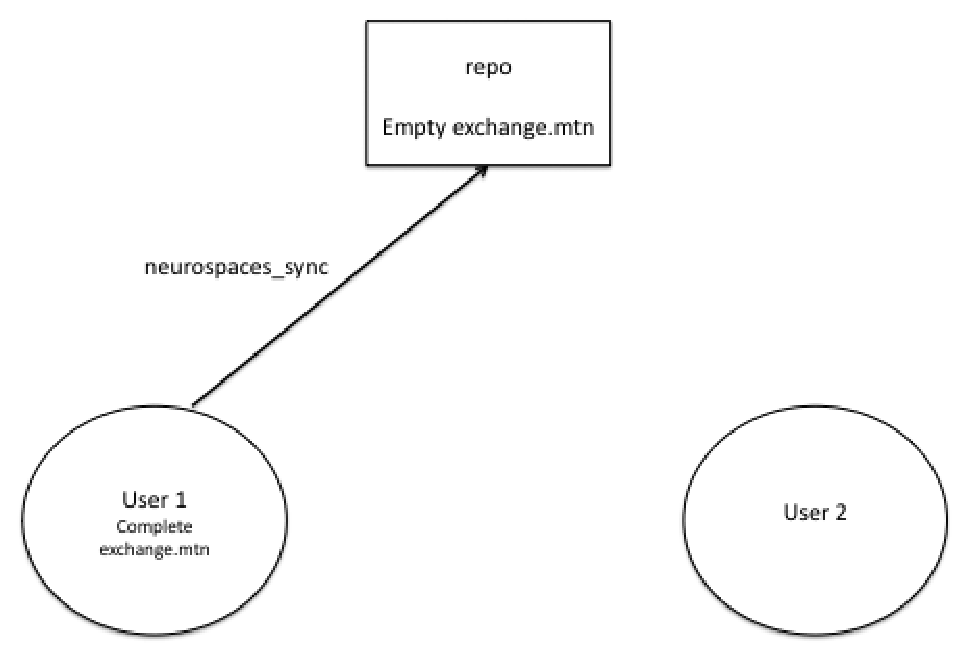
\includegraphics[scale=0.5]{figures/repo2.eps}
%   \caption{ }
   \label{fig:R2}
\end{figure}

{\tt User1} performs a {\it sync}, which pushes all code revisions to the repo exchange repository.

\begin{figure}[h]
\centering
   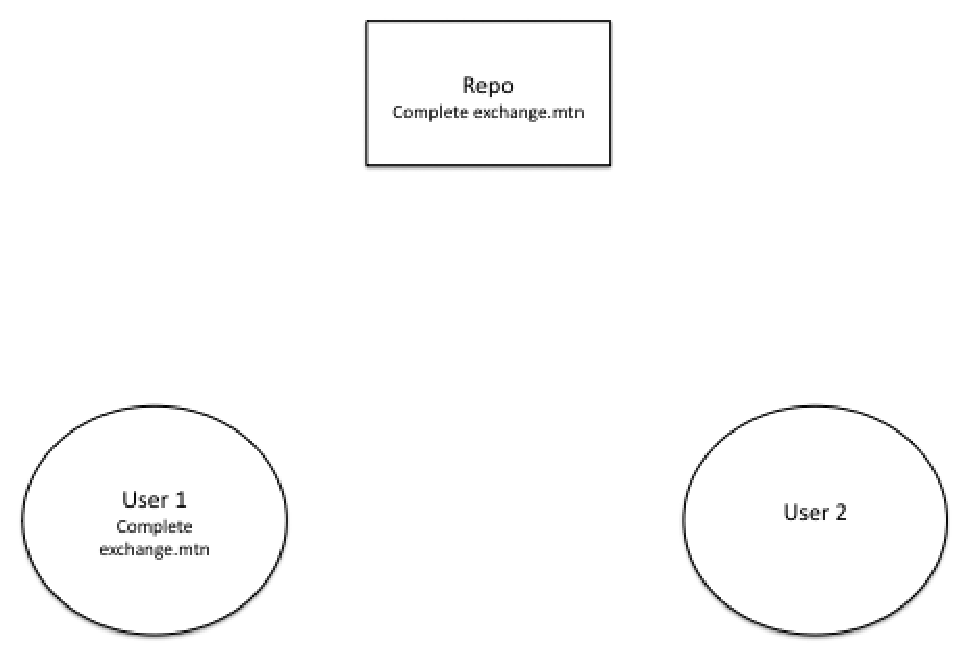
\includegraphics[scale=0.5]{figures/repo3.eps}
%   \caption{ }
   \label{fig:R3}
\end{figure}

The repo now has a complete set of code for the exchange package.

\begin{figure}[h]
\centering
   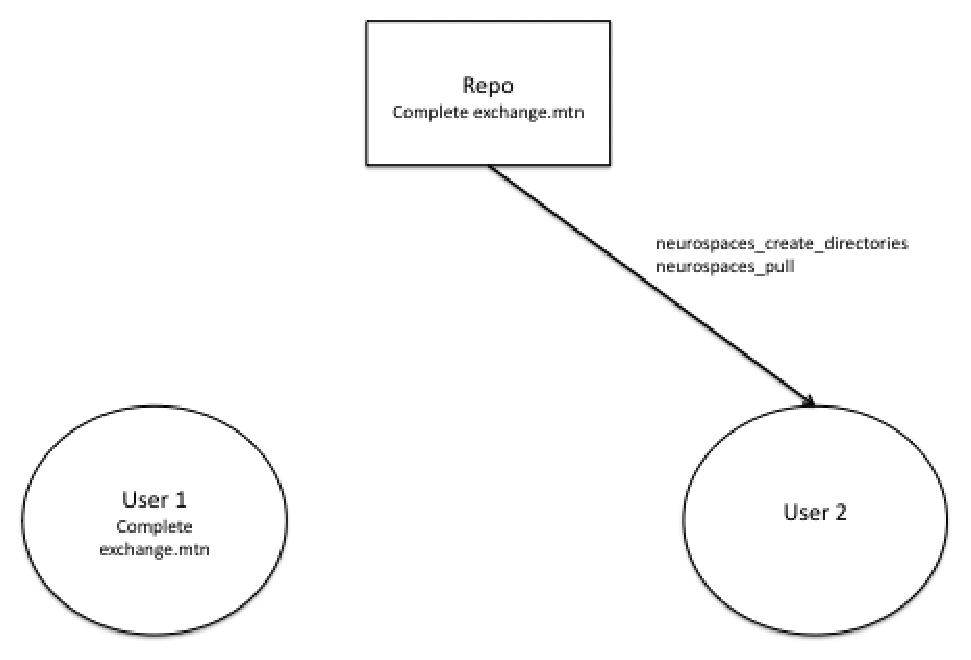
\includegraphics[scale=0.5]{figures/repo4.eps}
%   \caption{ }
   \label{fig:R4}
\end{figure}

{\tt User2} wants to download the {\it exchange} package, so they first perform a {\it neurospaces\_create\_directories} to create the checkout directories for source code. {\tt User2} can now perform a {\it pull}, which will automatically create their {\it exchange.mtn} repository in the correct location and make a connection to the repo to {\it pull} a complete set of source code revisions.

\begin{figure}[h]
\centering
   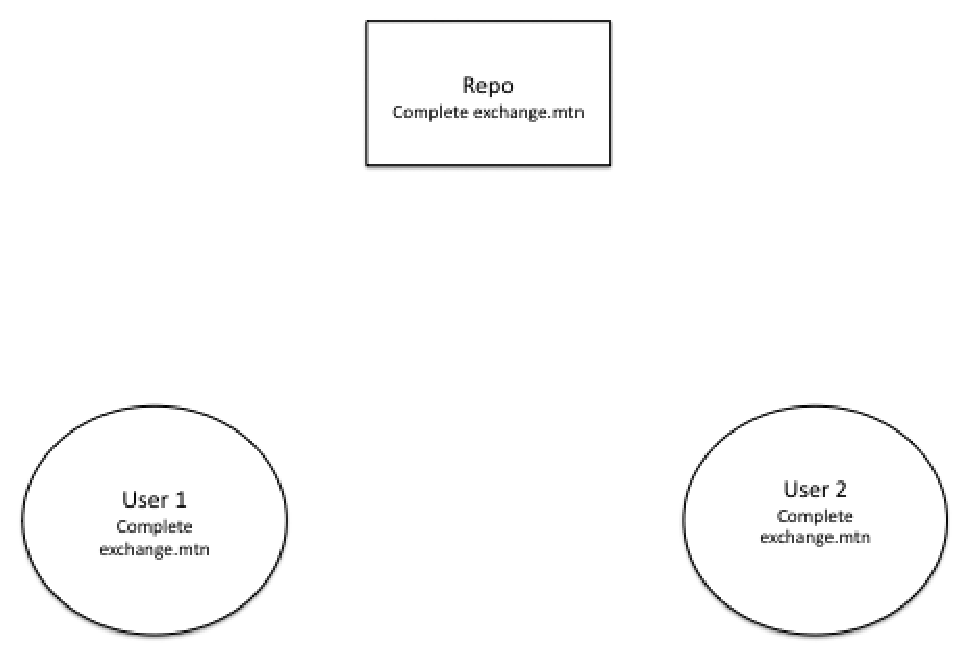
\includegraphics[scale=0.5]{figures/repo5.eps}
%   \caption{ }
   \label{fig:R5}
\end{figure}

Now {\tt User1} and {\tt User2} have a all code revisions and can collaborate work via the centralized repository.

\end{document}
